% Options for packages loaded elsewhere
\PassOptionsToPackage{unicode}{hyperref}
\PassOptionsToPackage{hyphens}{url}
\PassOptionsToPackage{dvipsnames,svgnames,x11names}{xcolor}
%
\documentclass[
  letterpaper,
  DIV=11,
  numbers=noendperiod]{scrreprt}

\usepackage{amsmath,amssymb}
\usepackage{iftex}
\ifPDFTeX
  \usepackage[T1]{fontenc}
  \usepackage[utf8]{inputenc}
  \usepackage{textcomp} % provide euro and other symbols
\else % if luatex or xetex
  \usepackage{unicode-math}
  \defaultfontfeatures{Scale=MatchLowercase}
  \defaultfontfeatures[\rmfamily]{Ligatures=TeX,Scale=1}
\fi
\usepackage{lmodern}
\ifPDFTeX\else  
    % xetex/luatex font selection
\fi
% Use upquote if available, for straight quotes in verbatim environments
\IfFileExists{upquote.sty}{\usepackage{upquote}}{}
\IfFileExists{microtype.sty}{% use microtype if available
  \usepackage[]{microtype}
  \UseMicrotypeSet[protrusion]{basicmath} % disable protrusion for tt fonts
}{}
\makeatletter
\@ifundefined{KOMAClassName}{% if non-KOMA class
  \IfFileExists{parskip.sty}{%
    \usepackage{parskip}
  }{% else
    \setlength{\parindent}{0pt}
    \setlength{\parskip}{6pt plus 2pt minus 1pt}}
}{% if KOMA class
  \KOMAoptions{parskip=half}}
\makeatother
\usepackage{xcolor}
\setlength{\emergencystretch}{3em} % prevent overfull lines
\setcounter{secnumdepth}{5}
% Make \paragraph and \subparagraph free-standing
\makeatletter
\ifx\paragraph\undefined\else
  \let\oldparagraph\paragraph
  \renewcommand{\paragraph}{
    \@ifstar
      \xxxParagraphStar
      \xxxParagraphNoStar
  }
  \newcommand{\xxxParagraphStar}[1]{\oldparagraph*{#1}\mbox{}}
  \newcommand{\xxxParagraphNoStar}[1]{\oldparagraph{#1}\mbox{}}
\fi
\ifx\subparagraph\undefined\else
  \let\oldsubparagraph\subparagraph
  \renewcommand{\subparagraph}{
    \@ifstar
      \xxxSubParagraphStar
      \xxxSubParagraphNoStar
  }
  \newcommand{\xxxSubParagraphStar}[1]{\oldsubparagraph*{#1}\mbox{}}
  \newcommand{\xxxSubParagraphNoStar}[1]{\oldsubparagraph{#1}\mbox{}}
\fi
\makeatother


\providecommand{\tightlist}{%
  \setlength{\itemsep}{0pt}\setlength{\parskip}{0pt}}\usepackage{longtable,booktabs,array}
\usepackage{calc} % for calculating minipage widths
% Correct order of tables after \paragraph or \subparagraph
\usepackage{etoolbox}
\makeatletter
\patchcmd\longtable{\par}{\if@noskipsec\mbox{}\fi\par}{}{}
\makeatother
% Allow footnotes in longtable head/foot
\IfFileExists{footnotehyper.sty}{\usepackage{footnotehyper}}{\usepackage{footnote}}
\makesavenoteenv{longtable}
\usepackage{graphicx}
\makeatletter
\def\maxwidth{\ifdim\Gin@nat@width>\linewidth\linewidth\else\Gin@nat@width\fi}
\def\maxheight{\ifdim\Gin@nat@height>\textheight\textheight\else\Gin@nat@height\fi}
\makeatother
% Scale images if necessary, so that they will not overflow the page
% margins by default, and it is still possible to overwrite the defaults
% using explicit options in \includegraphics[width, height, ...]{}
\setkeys{Gin}{width=\maxwidth,height=\maxheight,keepaspectratio}
% Set default figure placement to htbp
\makeatletter
\def\fps@figure{htbp}
\makeatother
% definitions for citeproc citations
\NewDocumentCommand\citeproctext{}{}
\NewDocumentCommand\citeproc{mm}{%
  \begingroup\def\citeproctext{#2}\cite{#1}\endgroup}
\makeatletter
 % allow citations to break across lines
 \let\@cite@ofmt\@firstofone
 % avoid brackets around text for \cite:
 \def\@biblabel#1{}
 \def\@cite#1#2{{#1\if@tempswa , #2\fi}}
\makeatother
\newlength{\cslhangindent}
\setlength{\cslhangindent}{1.5em}
\newlength{\csllabelwidth}
\setlength{\csllabelwidth}{3em}
\newenvironment{CSLReferences}[2] % #1 hanging-indent, #2 entry-spacing
 {\begin{list}{}{%
  \setlength{\itemindent}{0pt}
  \setlength{\leftmargin}{0pt}
  \setlength{\parsep}{0pt}
  % turn on hanging indent if param 1 is 1
  \ifodd #1
   \setlength{\leftmargin}{\cslhangindent}
   \setlength{\itemindent}{-1\cslhangindent}
  \fi
  % set entry spacing
  \setlength{\itemsep}{#2\baselineskip}}}
 {\end{list}}
\usepackage{calc}
\newcommand{\CSLBlock}[1]{\hfill\break\parbox[t]{\linewidth}{\strut\ignorespaces#1\strut}}
\newcommand{\CSLLeftMargin}[1]{\parbox[t]{\csllabelwidth}{\strut#1\strut}}
\newcommand{\CSLRightInline}[1]{\parbox[t]{\linewidth - \csllabelwidth}{\strut#1\strut}}
\newcommand{\CSLIndent}[1]{\hspace{\cslhangindent}#1}

\KOMAoption{captions}{tableheading}
\makeatletter
\@ifpackageloaded{bookmark}{}{\usepackage{bookmark}}
\makeatother
\makeatletter
\@ifpackageloaded{caption}{}{\usepackage{caption}}
\AtBeginDocument{%
\ifdefined\contentsname
  \renewcommand*\contentsname{Table of contents}
\else
  \newcommand\contentsname{Table of contents}
\fi
\ifdefined\listfigurename
  \renewcommand*\listfigurename{List of Figures}
\else
  \newcommand\listfigurename{List of Figures}
\fi
\ifdefined\listtablename
  \renewcommand*\listtablename{List of Tables}
\else
  \newcommand\listtablename{List of Tables}
\fi
\ifdefined\figurename
  \renewcommand*\figurename{Figure}
\else
  \newcommand\figurename{Figure}
\fi
\ifdefined\tablename
  \renewcommand*\tablename{Table}
\else
  \newcommand\tablename{Table}
\fi
}
\@ifpackageloaded{float}{}{\usepackage{float}}
\floatstyle{ruled}
\@ifundefined{c@chapter}{\newfloat{codelisting}{h}{lop}}{\newfloat{codelisting}{h}{lop}[chapter]}
\floatname{codelisting}{Listing}
\newcommand*\listoflistings{\listof{codelisting}{List of Listings}}
\makeatother
\makeatletter
\makeatother
\makeatletter
\@ifpackageloaded{caption}{}{\usepackage{caption}}
\@ifpackageloaded{subcaption}{}{\usepackage{subcaption}}
\makeatother
\ifLuaTeX
  \usepackage{selnolig}  % disable illegal ligatures
\fi
\usepackage{bookmark}

\IfFileExists{xurl.sty}{\usepackage{xurl}}{} % add URL line breaks if available
\urlstyle{same} % disable monospaced font for URLs
\hypersetup{
  pdftitle={Ecologie spatiale et régime alimentaire d'une espèce en danger critique d'extinction : apports pour la conservation du Vison d'Europe (Mustela lutreola) en France.},
  pdfauthor={Rémi Bodinier},
  colorlinks=true,
  linkcolor={blue},
  filecolor={Maroon},
  citecolor={Blue},
  urlcolor={Blue},
  pdfcreator={LaTeX via pandoc}}

\title{Ecologie spatiale et régime alimentaire d'une espèce en danger
critique d'extinction : apports pour la conservation du Vison d'Europe
(\emph{Mustela lutreola}) en France.}
\author{Rémi Bodinier}
\date{2024-06-19}

\begin{document}
\maketitle

\renewcommand*\contentsname{Table of contents}
{
\hypersetup{linkcolor=}
\setcounter{tocdepth}{2}
\tableofcontents
}
\bookmarksetup{startatroot}

\chapter*{Preface}\label{preface}
\addcontentsline{toc}{chapter}{Preface}

\markboth{Preface}{Preface}

Ce projet de thèse est réalisé par Rémi Bodinier au sein du GREGE
(Groupe de Recherche et d'Etude pour la Gestion de l'Environnement) en
co-direction avec le LBBE (Laboratoire de Biométrie et Biologie
Evolutive).

Le but de cette thèse est d'apporter des connaissances sur l'écologie du
Vison d'Europe à travers l'occupation de l'espace, l'utisation de
l'habitat, le régime alimentaire et les risques de collisions routières.
Grâce à cet apport de connaissances, le but de cette thèse est
d'améliorer les stratégies de conservation de l'espèce en milieu naturel
et de donner des critères pour de futures translocations d'individus
dans le milieu naturel.

Ce présent document est construit afin que les différentes personnes
impliquées dans ce projet de thèse puissent avoir un spport pour se
tenir au courant des avancées du projet.

\part{Introduction}

\chapter{Introduction générale}\label{introduction-guxe9nuxe9rale}

La récente et importante perte de biodiversité est un phénomène qui
suscite des inquiétudes de plus en plus nombreuses. Aussi alarmant, de
plus en plus d'espèces voient leur statut de conservation devenir chaque
année plus préoccupant (Ceballos et al., 2010) et le Vison d'Europe fait
partie de ces espèces dont le statut est particulièrement inquiétant. En
effet, cette espèce, considérée comme le mammifère carnivore le plus
menacé en Europe, est classée « en danger critique d'extinction » sur
les listes rouges mondiale (2011), européenne (2011), française (2017)
de l'UICN (MNHN, 2023). Les raisons de son déclin sont nombreuses mais
nous pouvons noter en particulier la mortalité accidentelle par
collisions routières qui joue aujourd'hui un rôle majeur en créant des
puits de mortalité locaux sur les derniers noyaux de population présents
(dans le cadre du premier PNA Vison, 69 spécimens découverts morts ont
été collectés dont 62\% (43) étaient victimes de collisions routières ;
Mission Vison d'Europe, 2003). Nous pouvons citer aussi la perte,
dégradation et fragmentation de ses habitats (Maran et Henttonen, 1995 ;
Lodé, 2001 ; DREAL et al., 2021), l'expansion d'une espèce exotique
envahissante, le Vison d'Amérique (Maran et al. (1998) ; Sidorovich,
2001 ; DREAL et al., 2021), ainsi que l'action de certains agents
pathogènes virulents (Fournier-Chambrillon et al., 2022). En 2007, on
estimait que ces menaces ont conduit à la perte de 85\% de l'aire de
répartition d'origine de l'espèce et plus de 90\% de ses effectifs
d'origine. En France, l'aire de répartition de l'espèce est passée de 38
départements à la fin du XIXème siècle à seulement sept au début du
XXIème (Figure 1) et le nombre d'individus encore en vie in natura est
estimé à moins de 250, faisant du Vison d'Europe une espèce très rare.
Afin de lutter contre la disparition de cette espèce, de nombreux
programmes ont vu le jour en France. Ce sont trois Plans Nationaux
d'Actions (PNA) sur les périodes 1999-2003 (DIREN et GREGE, 1999),
2007-2011 (DIREN et GEREA, 2007), et 2021-2031 (DREAL et al., 2021), un
Plan National d'Actions dit « intermédiaire » (PNAi) de 2015 à 2021
(DREAL et ONCFS, 2015), et deux projets européens de conservation, LIFE
VISON de 2017 à 2023 (LPO et al., 2017) et LIFE KANTAURIBAI de 2022 à
2027 (GAN-NIK et al., 2022) qui ont été mis en place et dont certains
sont encore en cours. Ces projets ont des envergures géographiques qui
peuvent différer, les PNA s'étendant sur 11 départements de trois
régions françaises (Nouvelle-Aquitaine : Charente, Charente-Maritime,
Dordogne, Gironde, Landes, Lot-et-Garonne, Pyrénées-Atlantiques,
Deux-Sèvres ; Occitanie : Gers, Hautes-Pyrénées ; Pays de la Loire :
Vendée), le LIFE VISON s'étendant sur huit sites Natura 2000 du bassin
de la Charente (départements de Charente et Charente-Maritime) et le
LIFE KANTAURIBAI sur 3 sites Natura 2000 du réseau hydrographique du
Golfe de Gascogne.

\begin{figure}[H]

{\centering 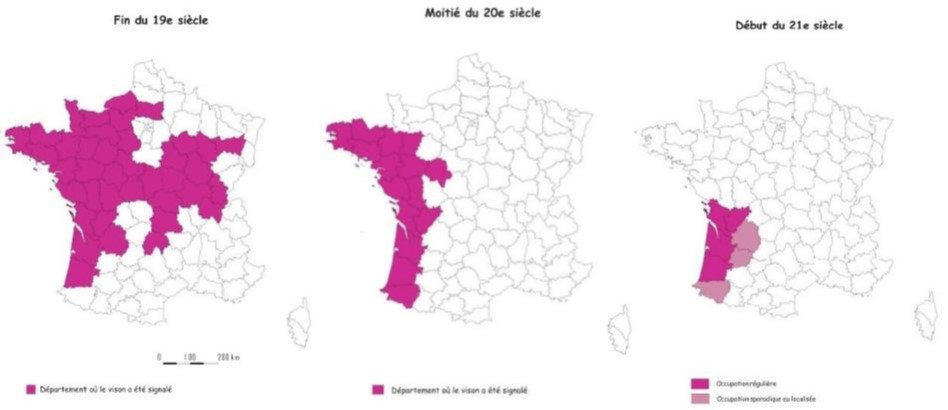
\includegraphics{image/evolution_repartition.jpg}

}

\caption{Evolution de l'aire de répartition du Vison d'Europe en France
(Bellefroid et Rosoux, 1998 ; Maizeret et al., 2002).}

\end{figure}%

Malgré la caractère très rare et cryptique de l'espèce, les
connaissances sur l'écologie spatiale et le régime alimentaire du Vison
d'Europe sont en partie documentées, mais certaines lacunes demeurent.
Le Vison d'Europe est un mammifère semi-aquatique qui change de gîte
quasi quotidiennement au sein de son grand domaine vital. En moyenne,
les distances parcourues par le Vison d'Europe entre deux localisations
journalières consécutives sont de l'ordre du kilomètre -- 0,4 kilomètres
pour les femelles et 1,8 kilomètres pour les mâles (S. Palazón and
Ruiz-Olmo (1998) ; Fournier et al. (2008) ; Cazaillon, 2021). Le sujet
nécessite cependant d'être approfondi, notamment dans l'état actuel très
dégradé des populations et avec des nouveaux outils d'analyses. En
particulier, des périodes correspondant aux variations de déplacements
n'ont pas été étudiées. Le domaine vital du Vison d'Europe s'étend sur
environ une dizaine de kilomètres de cours d'eau chez les mâles et moins
de la moitié pour les femelles (Garin et al. (2002) ; Ceña, 2003 ;
Fournier et al. (2008) ; Palomares, López-Bao, et al. (2017)). Aucune
donnée n'a cependant été publiée sur des individus évoluant en marais
littoraux comme ceux hébergeant les derniers noyaux populationnels
français. Les méthodes de modélisation surfacique du domaine vital les
plus couramment utilisées par les auteurs (méthode des Polygones
Convexes Minimums, MCP, ou méthode des Kernels) ne semblent pas adaptées
aux configurations linéaires des rivières, car elles ne prennent pas en
compte la sinuosité des cours d'eau. De plus, l'occupation fine de
l'espace, en particulier la notion de « zone coeur », est peu renseignée
pour cette espèce. La zone coeur correspondant à une zone fortement
utilisée et statistiquement plus utilisée que les zones fortement
utilisées dans l'hypothèse d'une occupation aléatoire de l'espace
(Powell, 2000). En ce qui concerne son habitat, le Vison d'Europe est
strictement inféodé aux zones humides, étant le plus souvent observé
dans des zones proches de l'eau (Palazón, 1998 ; Fournier et al., 2007).
L'espèce est connue pour gîter majoritairement dans la ripisylve lorsque
celle-ci est présente, avec des gîtes soit souterrains, soit au sol dans
la végétation dense comme les ronciers (Zabala et al. (2003) ; Fournier
et al. (2007) ; Palomares, Lopez-Bao, et al. (2017)). Ces connaissances
sur l'utilisation de l'habitat doivent cependant être approfondies.
Enfin, son régime alimentaire est constitué de micromammifères,
d'oiseaux, de poissons, d'amphibiens et d'invertébrés aquatiques dans
des proportions qui peuvent changer entre différents pays (Sidorovich et
al. (1998) ; Santiago Palazón, Ruiz-Olmo, and Gosàlbez (2004) ; S.
Palazón, Ruiz-Olmo, and Gosálbez (2008)), voire au sein d'une zone
définie (Santiago Palazón, Ruiz-Olmo, and Gosàlbez (2004)). Il n'existe
cependant aucune étude publiée du régime alimentaire du Vison d'Europe
en France et les études publiées dans d'autres pays ne prennent pas en
compte l'écologie spatiale du Vison d'Europe pour expliquer les
variations de régime alimentaire.

Dans ce contexte, le projet que nous souhaitons mener a pour objectif de
mettre à jour les connaissances sur l'écologie du Vison d'Europe, grâce
à de nouveaux protocoles et/ou de nouvelles méthodes d'analyses sur les
données déjà existantes. L'amélioration des connaissances sur la
mobilité de l'espèce permettra également d'estimer les facteurs
écologiques influençant les risques de collisions routières, facteur
majeur de surmortalité pour les derniers noyaux populationnels. Les
informations apportées par les nouvelles analyses menées permettront
d'orienter plus précisément les stratégies actuelles de conservation du
Vison d'Europe en France, dans son milieu naturel. Les résultats de ce
projet contribueront de surcroît à la définition des meilleures
conditions possibles requises pour de futures translocations d'individus
dans le milieu naturel.

\chapter{Synthèse bibliographique}\label{synthuxe8se-bibliographique}

\part{Méthodologie}

\chapter{Etude}\label{etude}

\section{Site d'étude}\label{site-duxe9tude}

Les données proviennent de trois aires d'études différentes : 1. la
vallée de la Charente en amont et en aval d'Angoulême dans le
département de Charente (16), à partir du suivi réalisé dans le cadre du
LIFE VISON entre 2020 et 2022 ; 1. les marais littoraux de Rochefort
dans le département de Charente-Maritime (17) à partir du suivi réalisé
dans le cadre du LIFE VISON entre 2020 et 2022 ; 1. les rivières des
Landes de Gascogne à partir d'individus suivis entre 1996 et 2000.

\begin{figure}[H]

{\centering 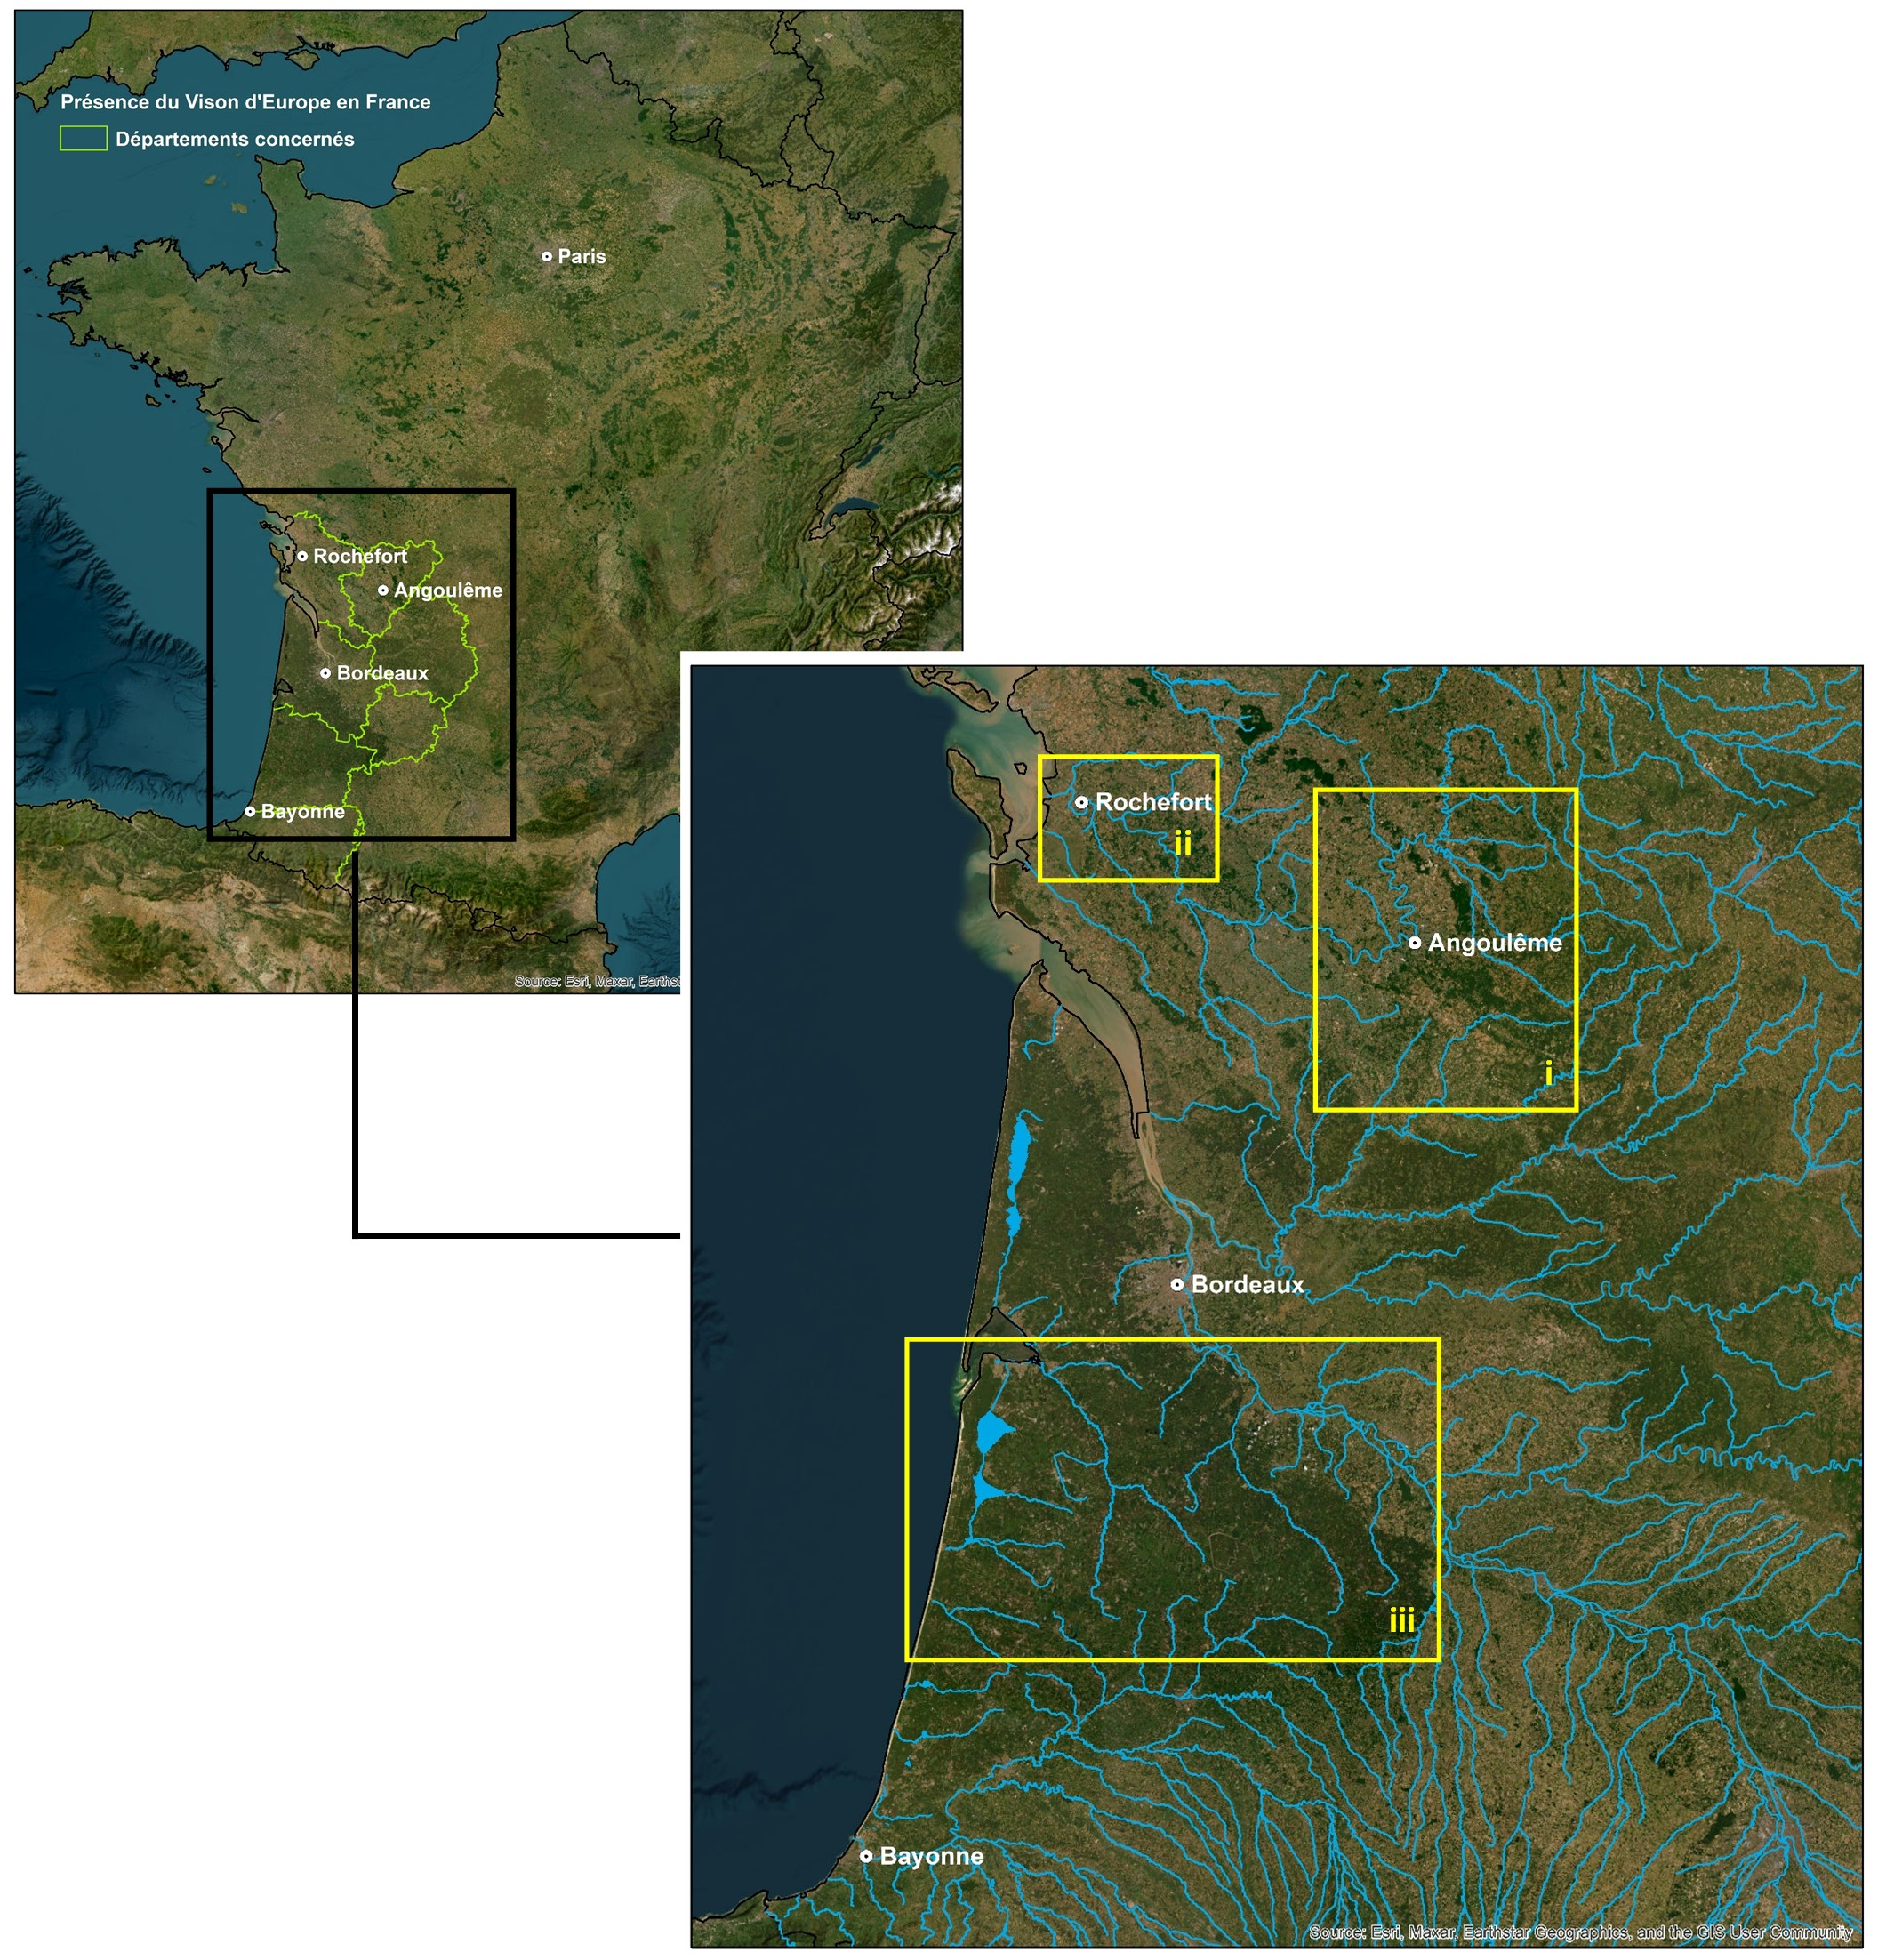
\includegraphics{image/zones_etudes.jpg}

}

\caption{Zones de collecte des données.}

\end{figure}%

\section{Radiopistage}\label{radiopistage}

Les individus ont été capturés par cages-pièges non vulnérantes lors de
sessions de capture impliquant dix nuitées consécutives de piégeage à
l'exception d'un individu qui a été capturé de façon accidentelle dans
une cage à Ragondins. Les individus capturés ont été équipés d'un
transpondeur sous-cutané permettant une identification pérenne. Un
sexage, un prélèvement de poils et une pesée ont également été faits au
même moment. Les sessions de capture ont été réalisées en dehors de la
période de mise-bas et d'élevage des jeunes, soit de début septembre à
fin mars.

Les individus capturés ont fait l'objet d'une intervention chirurgicale
pour être équipés d'un implant intraabdominal émetteur VHF (TELONICS ©)
s'ils correspondaient à certains critères morphologiques confirmant leur
bon état de santé (poids minimum de 520 grammes (g) pour les femelles et
875g pour les mâles en début d'année ou 500g pour les femelles et 800g
pour les mâles à l'automne). Un vétérinaire a réalisé l'intervention
pour placer l'émetteur VHF dans la cavité péritonéale des individus,
alors sous anesthésie générale. Les individus ont également reçu une
injection d'anti-douleur, d'anti-inflammatoire et d'antibiotique longue
action préventif (Fournier-Chambrillon et al., 2003). Ils ont été
relâchés environ 24 heures après la capture. Il est important de
préciser que les deux projets sur lesquels s'appuie la thèse ont fait
l'objet d'autorisations de captures et manipulations du Vison d'Europe
(autorisations n°96/363, 96/364, et 98/488 à 98/500 délivrées par le
Ministère en charge de l'Environnement dans le cadre du suivi dans les
Landes de Gascogne et arrêté portant dérogation à la protection stricte
des espèces du Ministère de la Transition Ecologique et Solidaire daté
du 19 avril 2018 pour le projet LIFE VISON) ainsi que dans le cadre du
LIFE VISON, conformément à la réglementation en place depuis 2013, une
autorisation de projet numéro APAFIS\#15599-2018062011206645 v2.

Les individus ont ensuite été suivis par radiopistage sur le principe de
la télémétrie (Janeau, 1994). Le signal sonore de l'émetteur est capté
par un récepteur WildLife Materials TRX 2000. Le radiopistage a été
organisé en deux parties. La première consiste à rechercher le signal en
véhicule équipé d'un mât télescopique (EUROMAST) muni à sa base d'un
pointeau permettant d'orienter sa position par rapport à un rapporteur
circulaire (de 0 à 360°). Le récepteur est, dans cette première
approche, relié à une antenne directionnelle Yagi cinq ou sept brins
fixée au mât. Lorsque le signal est perçu, la position de l'animal est
estimée sur la base d'une triangulation. Une fois cette triangulation
effectuée, la seconde partie consiste en une approche pédestre avec un
récepteur relié à une antenne à main Yagi deux ou trois brins
(TELONICS). Le but de cette approche pédestre est d'identifier la
localisation précise de l'individu correspondant à l'identification du
gîte diurne.

\section{Données acquises}\label{donnuxe9es-acquises}

Les données collectées sont donc des localisations quotidiennes précises
des individus, en journée, qui correspondent le plus souvent à des gîtes
diurnes. Tous les gîtes diurnes identifiés par approche pédestre ont été
décrits selon plusieurs paramètres environnementaux comme la typologie
de gîtes (au sol, dans une cavité, dans un tronc\ldots), la distance à
l'eau et le type d'eau proche (cours d'eau, plan d'eau, inondation), le
type de lit mineur le plus proche (fossé, bras courant, bras mort) ou
encore le recouvrement de différentes strates végétales environnantes.
En tout chaque gîte est décrit par sept variables.

Toutefois, l'approche pédestre était parfois impossible (individu sur
une île\ldots) et la localisation quotidienne associée est définie
uniquement à partir de la triangulation faite en voiture. Enfin, lorsque
l'intensité du signal sonore était fortement irrégulière, les animaux
ont été considérés comme étant en activité, la localisation étant
définie de la même manière que pour les gîtes pour lesquels il n'y a pas
eu d'approche pédestre.

En outre, pour le radiopistage réalisé dans les Landes de Gascogne, des
suivis continus des individus lors des phases d'activité ont été
réalisés à l'aide de deux véhicules positionnant l'animal en simultané
toutes les 10 minutes par triangulation. Ces suivis permettront de
qualifier les surfaces et habitats exploités lors des activités de
chasse et d'appliquer des approches méthodologiques liées à l'étude des
trajectoires individuelles.

Dans les Landes de Gascogne, neuf individus ont été suivis, dont deux
sur deux périodes différentes. En ce qui concerne le LIFE VISON, quatre
individus ont été suivis par radiopistage dans les marais de Rochefort
et quatre dans la vallée de la Charente. Trois de ces individus ont
d'ailleurs été suivis sur deux périodes différentes (Tableau 1). Un
dernier individu capturé accidentellement dans une cage à Ragondins en
Charente sur un sous-affluent de la Dordogne a également été suivi dans
le cadre du LIFE VISON.

\section{Collecte de crottes et régime
alimentaire}\label{collecte-de-crottes-et-ruxe9gime-alimentaire}

La découverte fortuite de crottes de Vison d'Europe dans le milieu
naturel est quasiment impossible. C'est pourquoi, leur collecte a été
organisée à partir de la recherche autour des gîtes des visons suivis
par radiopistage. Ainsi, après que l'individu a quitté son gîte et dans
les jours suivants la localisation précise d'un gîte diurne par
radiopistage, des crottes ont été cherchées dans un rayon de moins de 5
mètres autour des gîtes identifiés. Au total sur les deux projets, ce
sont 1347 échantillons qui ont été récoltés (Tableau 1). Etant donné le
grand nombre de crottes collectées et la difficulté de recherche dans le
milieu naturel, il n'est pas envisagé de récolter de nouveaux
échantillons dans ce projet de thèse.

Lors du suivi dans les Landes de Gascogne, 1011 crottes ont été
prélevées. La composition des crottes a été évaluée par identification
macroscopique et microscopique des résidus contenus (poils,
ossements\ldots).

Pour définir la composition du régime alimentaire dans le cadre du LIFE
VISON, les 336 crottes collectées ont été analysées en partenariat avec
le laboratoire GeCoLab de l'Université de Liège selon une méthode de «
metabarcoding ». Cette méthode repose sur l'amplification et le
séquençage à haut débit de type Nextseq de courts fragments très
variables du gène cytochrome oxydase 1 (CO1) contenu dans les
échantillons mis à l'analyse. Les fragments d'ADN séquencés pour chaque
échantillon sont ensuite comparés par une approche de type « blast » aux
bases de données publiques disponibles, notamment les bases de données
GENBANK et BOLD (Barcoding of Life), et à la base de données privée
GeCoLab pour les Mammifères. Ainsi, le Vison d'Europe est confirmé comme
espèce hôte et son régime alimentaire est révélé en identifiant toutes
les proies de vertébrés et d'invertébrés contenues dans ses fèces.

Afin d'obtenir des données de disponibilité en proies, il est envisagé
de faire des inventaires des différents types de proies sur les zones où
ont été suivis les différents individus. Dans tous les cas, une
recherche bibliographique devrait permettre de donner des premières
indications quant à la présence de chaque proie au sein des zones
d'études.

\chapter{Analyses présenties lors de la création de la
thèse}\label{analyses-pruxe9senties-lors-de-la-cruxe9ation-de-la-thuxe8se}

\section{Occupation de l'espace}\label{occupation-de-lespace}

Les domaines vitaux de tous les individus seront modélisés grâce à des
nouvelles méthodes qui n'ont pas été utilisées jusqu'à présent pour le
Vison d'Europe (Local Convex Hull (LoCoH), ponts browniens\ldots), à
partir des localisations quotidiennes de chaque individu. Les surfaces
occupées ainsi estimées par chacune des modélisations seront comparées
avec celles des modélisations les plus communément utilisées par les
auteurs ayant travaillé sur l'espèce (MCP, Kernels). L'analyse devrait
permettre de proposer la meilleure méthode à retenir pour la
modélisation des domaines vitaux du Vison d'Europe, tout en tenant
compte de la configuration bien différente des zones de marais et des
vallées alluviales sinueuses. Les domaines vitaux seront ensuite
analysés en fonction des caractéristiques des individus (sexe, classe
d'âge, statut reproducteur\ldots) par modèles mixtes en première
intention car en effet ces modèles devront prendre en compte comme
variable aléatoire entre autres la différence de temporalité entre les
deux projets mais aussi d'autres facteurs temporaires (saisons\ldots).
Des tests subsidiaires de choix de modèle (Critère d'Information
d'Akaike\ldots) viendront compléter les analyses. La modélisation des
surfaces exploitées sera également étudiée en fonction de la dispersion
spatiale des localisations, afin de définir des zones plus ou moins
utilisées au sein du domaine vital. Ces approches devraient donc
permettre de mettre en évidence des « zones coeurs », c'est-à-dire des
surfaces statistiquement plus utilisées que les zones fortement
utilisées dans l'hypothèse d'une utilisation aléatoire de l'espace
(Powell, 2000).

\section{Patrons de déplacements}\label{patrons-de-duxe9placements}

Grâce aux suivis continus des individus dans les Landes de Gascogne, une
étude de la trajectométrie pourra être faite afin de décrire des
typologies de déplacements selon les différentes phases d'activité
(chasse, déplacement entre gîte, \ldots). Les modèles utilisés pour
décrire ces phases d'activité devront prendre en compte certaines
caractéristiques des individus (âge, sexe, statut reproducteur, \ldots)
et certaines caractéristiques spatiales relevées lors de la partie i. La
mobilité individuelle sera également étudiée d'une autre manière à
partir des données qui correspondent aux localisations quotidiennes. En
effet, Laundré et al.~(1987) ont montré qu'utiliser des distances entre
localisations relevées à un jour d'intervalle présentaient certains
problèmes en tant qu'indicateur du trajet et des mouvements totaux d'un
individu. De la trajectométrie ne peut donc pas être fait avec ces
données et l'étude de la mobilité individuelle à partir des
localisations quotidiennes sera donc menée en utilisant comme indicateur
les distances entre deux localisations diurnes relevées à un jour
d'intervalle. La modélisation de cet indicateur se fera en projetant
chaque gîte sur l'axe médian du lit majeur du cours d'eau utilisé et en
calculant la distance entre le gîte d'un jour et celui de la veille en
suivant cet axe médian. Cette méthode est proposée pour venir se
substituer aux distances euclidiennes, afin de mieux correspondre à la
réalité du terrain et à la sinuosité des cours d'eau. Ensuite, les
distances seront comparées sur des échelles temporelles différentes
(jour, semaine, mois, saison\ldots). Les distances seront aussi
comparées en fonction du sexe, voire de l'âge et du statut reproducteur.
De la même manière que pour l'étude de l'occupation de l'espace, les
analyses seront des modèles prenant en compte les différentes variables
d'influence, complétées par des analyses de choix de modèles. Ainsi, des
périodes de plus ou moins forte mobilité seront définies et pourront
être reliées à certains évènements (rut, reproduction, élevage des
jeunes\ldots). Afin de pouvoir relier les variations des distances
parcourues et les évènements écologiques cités juste avant, il faudra
prendre en compte les gîtes de reproduction dans cette étude. Ces
périodes pourront être définies comme des périodes écologiques de
l'espèce. En outre, la mobilité au sein des différentes parties des
domaines vitaux sera également étudiée grâce aux résultats de la partie
i.

\section{Utilisation de l'habitat}\label{utilisation-de-lhabitat}

Il s'agira d'identifier les habitats utilisés et ceux sélectionnés par
l'espèce pour installer ses gîtes diurnes grâce à la cartographie de
l'occupation du sol réalisée. Deux approches complémentaires seront
menées : 1) analyser les modalités d'utilisation des habitats en
comparant les distributions des gîtes par habitat grâce à une analyse
multivariée en composantes, 2) définir les sélections d'habitats en
comparant en première intention les habitats des localisations à la
disponibilité présente dans le domaine vital, c'est-à-dire une sélection
du 3ème ordre (sensu Johnson, 1980). Les analyses seront faites grâce à
une approche de type k-select (Calenge et al., 2005). L'utilisation et
la sélection des habitats seront également analysées en fonction des
caractéristiques des individus (sexe, classe d'âge, statut
reproducteur\ldots). De plus, une analyse temporelle pourra être menée
en utilisant entre autres les périodes définies lors de l'analyse de la
mobilité (partie ii.). En outre, les compositions en habitats au sein
des différentes surfaces décrites lors des analyses de l'occupation de
l'espace (partie i.) mais aussi lors de la description des surfaces de
chasse dans l'étude de la mobilité (partie ii.) seront également
étudiées. Une analyse spatiale de l'utilisation et de la sélection des
habitats sera ainsi menée. Dans cette partie, les gîtes de repos et les
gîtes de mises bas et d'élevage des jeunes ne seront pas approchés de la
même façon, le choix du gîte de reproduction impliquant des critères
différents (sécurité des jeunes, \ldots). Une analyse descriptive de
l'habitat utilisé pour installer le gîte de reproduction sera ainsi
menée en parallèle, étant donné le faible nombre de gîtes de
reproduction identifiés.

\section{Caractéristiques des
gîtes}\label{caractuxe9ristiques-des-guxeetes}

Il s'agira d'identifier les caractéristiques préférées dans
l'établissement du gîte diurne. A partir des paramètres environnementaux
relevés à une échelle fine sur chacun des gîtes identifiés par approche
pédestres et cités dans la méthodologie, la préférence de certains de
ces paramètres sera analysée selon les caractéristiques des individus
(sexe, classe d'âge, statut reproducteur\ldots). L'analyse devra
également prendre en compte l'habitat dans lequel se situe le gîte
diurne afin de relever de potentiels correspondances entre les deux
variables. Une analyse multivariée de type canonique est pensée comme
première approche (analyse procustéenne ou analyse de co-inertie).
Enfin, des facteurs temporels (périodes définies lors de l'analyse de la
mobilité partie ii.) et spatiaux (surfaces décrites dans l'étude de
l'occupation de l'espace partie i.) devront être pris en compte pour
expliquer les choix de certaines caractéristiques. De même que dans
l'étude de l'habitat, les gîtes de repos et les gîtes de mises bas et
d'élevage des jeunes ne seront pas approchés de la même façon. Une
analyse descriptive des caractéristiques préférées pour installer le
gîte de reproduction sera ainsi menée en parallèle, pour les mêmes
raisons que pour l'étude de l'habitat.

\section{Régime alimentaire}\label{ruxe9gime-alimentaire}

Pour finir, le régime alimentaire sera étudié grâce aux analyses de la
composition de crottes récoltées sur les gîtes identifiés lors du
radiopistage. Dans un premier temps, des indices de diversité ou de
richesse (basé sur les indices de Shannon et de Simpson) seront calculés
pour chacune des crottes et ces indices seront comparés au sein des
habitats (partie iii.) et des surfaces (partie i.) dans lesquels les
crottes sont trouvées. Le Vison d'Europe pouvant chasser entre deux
gîtes diurnes, une attention particulière devra être porté à l'échelle à
laquelle se feront les analyses. De plus, les études actuelles semblent
montrer que cette espèce est généraliste, il faudra donc mettre en avant
les habitats ou les surfaces dans lesquels les indices montrent une
grande diversité d'espèces voire des taxons supérieurs. Ensuite, et sur
le même principe que pour l'habitat, l'étude du régime alimentaire
tentera de mettre en avant une sélection de certaines proies par les
différents individus selon la ressource disponible dans le domaine
vital. Il s'agira de comparer les disponibilités en proies relevées lors
des inventaires aux proportions de proies retrouvées dans les fèces par
une approche s'inspirant des méthodes analytiques de sélection des
habitats (k-select, eigenanalysis, \ldots). L'individu, le sexe et l'âge
seront des variables à prendre en compte pour expliquer une potentielle
sélection. Cette comparaison devra également prendre en compte la
période (résultats de la partie ii.) puisque les proies du Vison
d'Europe n'ont pas toutes la même écologie. Enfin, les crottes ayant été
localisées, il est possible d'observer des différences de proies
sélectionnées en fonction de la localisation au sein du domaine vital
(dans ou hors zone coeur définies en partie i.).

\section{Risque de collisions
routières}\label{risque-de-collisions-routiuxe8res}

Pour cette analyse, des variables permettant d'estimer un risque de
collision devront tout d'abord être identifiées. Ces variables prendront
en compte les résultats des analyses précédentes mais pas seulement. En
effet le premier type de variable se concentrera sur les composantes
anthropiques (trafic routier sur le franchissement, distance au prochain
franchissement le plus proche\ldots). L'autre type de variables
concernera des variables environnementales définies à partir des
analyses précédentes, en particulier les résultats de l'analyse de
l'utilisation de l'habitat partie iii (présence/absence d'habitats
favorables dans un rayon défini par la mobilité journalière,
présence/absence d'habitats favorables des deux côtés du franchissement
et distance à ceux-ci\ldots). Une analyse précise des collisions
routières recensées lors des différents projets permettra d'associer à
chacune des collisions des valeurs pour chacun des variables retenues.
Une analyse multivariée en composante (analyse des correspondances
multiples ou analyse mixte) permettra ensuite d'expliquer les facteurs
principaux expliquant la mortalité par collision routière.

\chapter{Methodologie de l'étude de l'occupation de
l'espace}\label{methodologie-de-luxe9tude-de-loccupation-de-lespace}

\section{Objectifs de l'étude}\label{objectifs-de-luxe9tude}

Cette étude a pour objectif de connaître plus en détails les modalités
d'occupation de l'espace, ainsi que d'établir des variables explicatives
pour les axes suivant.

Qui plus est, les objectifs de cette partie devront répondre au but de
la thèse qui est d'améliorer la stratégie de conservation des individus
dans le milieu naturel ainsi que de dresser des critères pour
l'établissement de zones propices à la translocation d'individus
d'élevage dans le milieu naturel.

Ainsi les objectifs seront de : - Connaître les surfaces ou les
linéaires à protéger lors de la conservation de l'espèce ainsi que les
espaces prévisionnels à couvrir lors du relâcher des individus
transloqués. - Identifier des zones plus utilisées que d'autres au sein
du domaine vital, ce qui est appelé ``zones coeurs'' dans la
littérature. Ces zones coeurs seront utilisées dans la partie sur
l'utilisation des habitats, en comparant les habitats en et hors zones
coeurs.

POur remplir ces objectifs, plusieurs méthodes sont prévues.

\section{Méthodes utilisées}\label{muxe9thodes-utilisuxe9es}

\subsection{Km linéaire}\label{km-linuxe9aire}

Pour la plupart des études ayant portées sur des espèces inféodés à un
milieu linéaire comme le sont les cours d'eau, le domaine vital est
souvent calculé comme la distance de cours d'eau entre la localisation
la plus en aval et celle la plus en amont. Les zones coeurs pourraient
être des portions de ce linéaire où l'individu s'arrête plus souvent que
sur d'autres. POur les identifier, il faut calculer la distance entre un
des points extrêmes (localisation la plus en aval ou la plus en amont)
et chacune des localisations, via le cours d'eau. Il faut ensuite
observer la distribution de ces distances. La courbe que la distribution
va former devrait présenter un ou des pics pouvant être associés à des
zones coeurs. Par exemple, si la distribution forme une coure de Gauss,
la zone coeur est compris entre la distance au premier quartile et la
distance au troisième quartile.

Cependant cette méthode ne permettra pas de pouvoir comparer des
habitats puisu'il est associé à une seul type d'habitat : le cours
d'eau. Ils font donc alors trouver une méthode surfacique.

\subsection{Km linéaire tampon}\label{km-linuxe9aire-tampon}

On pourrait réutiliser le cours d'eau en la localisatio la plus en aval
et celle la plus en amont, en ajoutant un tampon au cours d'eau. Ce
tampon serait créé en mesurant toutes les distances entre les
localisations et le cours d'eau le plus proche. La valeur du tampon est
alors la distance maximale entre les localisations et le cours d'eau,
par individu.

\subsection{Kernel}\label{kernel}

Une méthode de modélisation du domaine vital très utilisée est la
méthode des Kernel. En prenant comme zone coeur les kernel 50\%.
Cependant, la configuration des cours d'eau dans notre étude va
fortement surestimer la taille du domaine vital en utilisant cette
techniques. Il faut donc utiliser une variante du Kernel qui permettra
de prendre en compte la réalité du terrain et les spécificités
écologiques du Vison d'Europe.

\section{Comparaison des méthodes}\label{comparaison-des-muxe9thodes}

Les méthodes seront toutes appliquées à notre jeu de données. De plus
les déterminismes de la taille du domaine vital seront analysés pour
chacune des méthodes. Ainsi il faudra observe si ce sont toujours les
mêmes déterminismes qui influencent la taille du domain vital. De plus,
avoir plusieurs méthodes de modélisation du domaine vital permettra
aussi d'estimer celui-ci comme un intervalle entre deux surfaces et pas
comme une surface ``fixe''.

\chapter{Méthodologie de l'étude de l'utilisation des
habitats}\label{muxe9thodologie-de-luxe9tude-de-lutilisation-des-habitats}

\part{Résultats}

\chapter{Résultats de l'étude de l'occupation de
l'espace}\label{ruxe9sultats-de-luxe9tude-de-loccupation-de-lespace}

\bookmarksetup{startatroot}

\chapter*{References}\label{references}
\addcontentsline{toc}{chapter}{References}

\markboth{References}{References}

\phantomsection\label{refs}
\begin{CSLReferences}{1}{0}
\bibitem[\citeproctext]{ref-fournier_spatial_2008}
Fournier, Pascal, Christian Maizeret, Christine Fournier-Chambrillon,
Nicolas Ilbert, Stéphane Aulagnier, and François Spitz. 2008. {``Spatial
Behaviour of {European} {minkMustela} Lutreola and {polecatMustela}
Putorius in Southwestern {France}.''} \emph{Mammal Research} 53 (4):
343--54. \url{https://doi.org/10.1007/BF03195195}.

\bibitem[\citeproctext]{ref-fournier_habitat_2007}
Fournier, Pascal, Christian Maizeret, David Jimenez, Jean-Pierre
Chusseau, Stéphane Aulagnier, and François Spitz. 2007. {``Habitat
Utilization by Sympatric {European} {minkMustela} Lutreola and
{polecatsMustela} Putorius in South-Western {France}.''} \emph{Acta
Theriologica} 52 (1): 1--12. \url{https://doi.org/10.1007/BF03194194}.

\bibitem[\citeproctext]{ref-garin_home_2002}
Garin, Inazio, Inigo Zuberogoitia, Jabi Zabala, Joxerra Aihartza,
Anthony P. Clevenger, and Ana Rallo. 2002. {``Home Ranges of {European}
{minkMustela} Lutreola in Southwestern {Europe}.''} \emph{Acta
Theriologica} 47 (1): 55--62. \url{https://doi.org/10.1007/BF03193566}.

\bibitem[\citeproctext]{ref-maran_diet_1998}
Maran, T., H. Kruuk, D. W. Macdonald, and M. Polma. 1998. {``Diet of Two
Species of Mink in {Estonia}: Displacement of \emph{{Mustela} Lutreola}
by \emph{{M}. Vison}.''} \emph{Journal of Zoology} 245 (2): 218--22.
\url{https://doi.org/10.1111/j.1469-7998.1998.tb00093.x}.

\bibitem[\citeproctext]{ref-palazon_diet_2004}
Palazón, Santiago, J. Ruiz-Olmo, and J. Gosàlbez. 2004. {``Diet of
{European} Mink ( \emph{{Mustela} Lutreola} ) in {Northern} {Spain}.''}
\emph{Mamm} 68 (2-3): 159--65.
\url{https://doi.org/10.1515/mamm.2004.016}.

\bibitem[\citeproctext]{ref-dunstone_preliminary_1998}
Palazón, S., and J. Ruiz-Olmo. 1998. {``A Preliminary Study of the
Behaviour of the {European} Mink \emph{{Mustela} Lutreola} in {Spain},
by Means of Radiotracking.''} In \emph{Behaviour and {Ecology} of
{Riparian} {Mammals}}, edited by Nigel Dunstone and Martyn L. Gorman,
93--106. \url{https://doi.org/10.1017/CBO9780511721830.007}.

\bibitem[\citeproctext]{ref-palazon_autumn-winter_2008}
Palazón, S., J. Ruiz-Olmo, and J. Gosálbez. 2008. {``Autumn-Winter Diet
of Three Carnivores, {European} Mink ({Mustela} Lutreola), {Eurasian}
Otter ({Lutra} Lutra) and Small-Spotted Genet ({Genetta} Genetta), in
Northern {Spain}.''} \emph{Animal Biodiversity and Conservation} 31 (2):
37--43. \url{https://doi.org/10.32800/abc.2008.31.2.0037}.

\bibitem[\citeproctext]{ref-palomares_resting_2017}
Palomares, Francisco, Jose Lopez-Bao, Garbine Telletxea, Juan Ceña,
Pascal Fournier, Gloria Giralda, and Fermin Urra. 2017. {``Resting and
Denning Sites of {European} Mink in the Northern {Iberian} {Peninsula}
({Western} {Europe}).''} \emph{Hystrix, the Italian Journal of
Mammalogy} 28 (1). \url{https://doi.org/10.4404/hystrix-28.1-12298}.

\bibitem[\citeproctext]{ref-palomares_activity_2017}
Palomares, Francisco, J. V. López-Bao, G. Telletxea, J. C. Ceña, P.
Fournier, G. Giralda, and F. Urra. 2017. {``Activity and Home Range in a
Recently Widespread {European} Mink Population in {Western} {Europe}.''}
\emph{European Journal of Wildlife Research} 63 (5): 78.
\url{https://doi.org/10.1007/s10344-017-1135-0}.

\bibitem[\citeproctext]{ref-dunstone_diets_1998}
Sidorovich, V., H. Kruuk, D. W. Macdonald, and T. Maran. 1998. {``Diets
of Semi-Aquatic Carnivores in Northern {Belarus}, with Implications for
Population Changes.''} In \emph{Behaviour and {Ecology} of {Riparian}
{Mammals}}, edited by Nigel Dunstone and Martyn L. Gorman, 1st ed.,
177--90. Cambridge University Press.
\url{https://doi.org/10.1017/CBO9780511721830.012}.

\bibitem[\citeproctext]{ref-zabala_landscape_2003}
Zabala, Jabi, Iñigo Zuberogoitia, Inazio Garin, and Joxerra Aihartza.
2003. {``Landscape Features in the Habitat Selection of {European} Mink
({Mustela} Lutreola) in South-Western {Europe}.''} \emph{Journal of
Zoology} 260 (4): 415--21.
\url{https://doi.org/10.1017/S0952836903003881}.

\end{CSLReferences}



\end{document}
